% !Mode:: "TeX:UTF-8"
\def\usewhat{pdflatex}                               % 定义编译方式 dvipdfmx 或者 pdflatex,默认为 dvipdfmx
                                                     % 方式编译,如果需要修改,只需改变花括号中的内容即可。
\documentclass[12pt,openright,a4paper,twoside]{book} %原本的设置
%\documentclass[12pt,openany,twoside]{book}           % 本科生毕业论文通常采用单页排版
% !Mode:: "TeX:UTF-8"
%  Authors: 张井   Jing Zhang: prayever@gmail.com     天津大学2010级管理与经济学部信息管理与信息系统专业硕士生
%           余蓝涛 Lantao Yu: lantaoyu1991@gmail.com  天津大学2008级精密仪器与光电子工程学院测控技术与仪器专业本科生

%%%%%%%%%% Package %%%%%%%%%%%%
\usepackage{graphicx}                       % 支持插图处理
\usepackage[a4paper,text={146.4true mm,239.2 true mm},top= 26.2true mm,left=31.8 true mm,head=6true mm,headsep=6.5true mm,foot=16.5true mm]{geometry}
                                            % 支持版面尺寸设置
\usepackage[squaren]{SIunits}               % 支持国际标准单位

\usepackage{titlesec}                       % 控制标题的宏包
\usepackage{titletoc}                       % 控制目录的宏包
\usepackage{fancyhdr}                       % fancyhdr宏包 支持页眉和页脚的相关定义
\usepackage[UTF8]{ctex}                     % 支持中文显示
\usepackage{CJKpunct}                       % 精细调整中文的标点符号
\usepackage{color}                          % 支持彩色
\usepackage{amsmath}                        % AMSLaTeX宏包 用来排出更加漂亮的公式
\usepackage{amssymb}                        % 数学符号生成命令
\usepackage[below]{placeins}    %允许上一个section的浮动图形出现在下一个section的开始部分,还提供\FloatBarrier命令,使所有未处理的浮动图形立即被处理
\usepackage{multirow}                       % 使用Multirow宏包,使得表格可以合并多个row格
\usepackage{booktabs}                       % 表格,横的粗线;\specialrule{1pt}{0pt}{0pt}
\usepackage{longtable}                      % 支持跨页的表格。
\usepackage{tabularx}                       % 自动设置表格的列宽
\usepackage{subfigure}                      % 支持子图 %centerlast 设置最后一行是否居中
\usepackage[subfigure]{ccaption}            % 支持子图的中文标题
\usepackage[sort&compress,numbers]{natbib}  % 支持引用缩写的宏包
\usepackage{enumitem}                       % 使用enumitem宏包,改变列表项的格式
\usepackage{calc}                           % 长度可以用+ - * / 进行计算
\usepackage{txfonts}                        % 字体宏包
\usepackage{bm}                             % 处理数学公式中的黑斜体的宏包
\usepackage[amsmath,thmmarks,hyperref]{ntheorem}  % 定理类环境宏包,其中 amsmath 选项用来兼容 AMS LaTeX 的宏包
\usepackage{CJKnumb}                        % 提供将阿拉伯数字转换成中文数字的命令
\usepackage{indentfirst}                    % 首行缩进宏包
\usepackage{CJKutf8}                        % 用在UTF8编码环境下,它可以自动调用CJK,同时针对UTF8编码作了设置
%\usepackage{hypbmsec}                      % 用来控制书签中标题显示内容
%\usepackage{enumerate}                      % 用于控制排序列表的编号样式
\newcommand{\tabincell}[2]{\begin{tabular}{@{}#1@{}}#2\end{tabular}}
\usepackage{xcolor}
%支持代码环境
\usepackage{listings}
\lstset{numbers=left,
language=[ANSI]{C},
numberstyle=\tiny,
extendedchars=false,
showstringspaces=false,
breakatwhitespace=false,
breaklines=true,
captionpos=b,
keywordstyle=\color{blue!70},
commentstyle=\color{red!50!green!50!blue!50},
frame=shadowbox,
rulesepcolor=\color{red!20!green!20!blue!20}
}
%支持算法环境
\usepackage[longend,linesnumbered,boxed,ruled,lined]{algorithm2e}
%\usepackage{algorithmic}

\usepackage{array}
\newcommand{\PreserveBackslash}[1]{\let\temp=\\#1\let\\=\temp}
\newcolumntype{C}[1]{>{\PreserveBackslash\centering}p{#1}}
\newcolumntype{R}[1]{>{\PreserveBackslash\raggedleft}p{#1}}
\newcolumntype{L}[1]{>{\PreserveBackslash\raggedright}p{#1}}

% 生成有书签的 pdf 及其生成方式。通常可以在 tjumain.tex 文件的第一行选择 pdflatex 或者是 dvipdfmx 编译手段。如果选择前者,则使用 pdflatex + pdflatex 编译; 如果选择后者,在编译的时候选择 latex + bibtex + latex + latex 编译。出现混淆的时候,系统会报错。
% 如果您的pdf制作中文书签有乱码使用如下命令,就可以解决了
\def\atemp{dvipdfmx}\ifx\atemp\usewhat
\usepackage[dvipdfmx,unicode,               % dvipdfmx 编译, 加入了中文复制,粘贴支持引擎。
            pdfstartview=FitH,
            bookmarksnumbered=true,
            bookmarksopen=true,
            colorlinks=false,
            pdfborder={0 0 1},
            citecolor=blue,
            linkcolor=black,
            anchorcolor=green,
            urlcolor=blue,
            breaklinks=true
            ]{hyperref}
\fi

\def\atemp{pdflatex}\ifx\atemp\usewhat
\usepackage{cmap}                           % pdflatex 编译时,可以生成可复制、粘贴的中文 PDF 文档, 缺点是在Windows上显示时效果不大好,字体发虚
\usepackage[pdftex,unicode,
            %CJKbookmarks=true,
            bookmarksnumbered=true,
            bookmarksopen=true,
            colorlinks=false,
            pdfborder={0 0 0},%pdfborder={0 0 1}就能显示红色框
            citecolor=blue,
            linkcolor=red,
            anchorcolor=green,
            urlcolor=blue,
            breaklinks=true
            ]{hyperref}
\fi

\usepackage{setspace}   % 用于目录设置行距


\usepackage{caption}

                                % 定义本文所使用宏包
\usepackage{graphicx}
\usepackage{subfigure}
\usepackage{epstopdf}                                 %支持eps图片转换成PDF格式
\usepackage{tipa}
\graphicspath{{figures/}}                            % 定义所有的 .eps 文件在 figures 子目录下
\begin{document}                                     % 开始全文
\begin{CJK*}{UTF8}{song}                             % 开始中文字体使用
% !Mode:: "TeX:UTF-8"

%%%%%%%%%%%%%%%%% Fonts Definition and Basics %%%%%%%%%%%%%%%%%
\newcommand{\song}{\CJKfamily{song}}    % 宋体
\newcommand{\fs}{\CJKfamily{fs}}        % 仿宋体
\newcommand{\kai}{\CJKfamily{kai}}      % 楷体
\newcommand{\hei}{\CJKfamily{hei}}      % 黑体
\newcommand{\li}{\CJKfamily{li}}        % 隶书
\newcommand{\chuhao}{\fontsize{28pt}{28pt}\selectfont}       % 初号, 单倍行距
\newcommand{\yihao}{\fontsize{26pt}{26pt}\selectfont}       % 一号, 单倍行距
\newcommand{\xiaoyi}{\fontsize{24pt}{24pt}\selectfont}      % 小一, 单倍行距
\newcommand{\erhao}{\fontsize{22pt}{1.25\baselineskip}\selectfont}       % 二号, 1.25 倍行距
\newcommand{\xiaoer}{\fontsize{18pt}{18pt}\selectfont}      % 小二, 单倍行距
\newcommand{\sanhao}{\fontsize{16pt}{16pt}\selectfont}      % 三号, 单倍行距
\newcommand{\xiaosan}{\fontsize{15pt}{15pt}\selectfont}     % 小三, 单倍行距
\newcommand{\sihao}{\fontsize{14pt}{14pt}\selectfont}       % 四号, 单倍行距
\newcommand{\xiaosi}{\fontsize{12pt}{12pt}\selectfont}      % 小四, 单倍行距
\newcommand{\wuhao}{\fontsize{10.5pt}{10.5pt}\selectfont}   % 五号, 单倍行距
\newcommand{\xiaowu}{\fontsize{9pt}{9pt}\selectfont}        % 小五, 单倍行距

\CJKtilde  % 重新定义了波浪符~的意义
\newcommand\prechaptername{第}
\newcommand\postchaptername{章}

\punctstyle{hangmobanjiao}             % 调整中文字符的表示,行内占一个字符宽度,行尾占半个字符宽度

% 调整罗列环境的布局
\setitemize{leftmargin=3em,itemsep=0em,partopsep=0em,parsep=0em,topsep=-0em}
\setenumerate{leftmargin=3em,itemsep=0em,partopsep=0em,parsep=0em,topsep=0em}

% 避免宏包 hyperref 和 arydshln 不兼容带来的目录链接失效的问题。
\def\temp{\relax}
\let\temp\addcontentsline
\gdef\addcontentsline{\phantomsection\temp}

% 自定义项目列表标签及格式 \begin{publist} 列表项 \end{publist}
\newcounter{pubctr} %自定义新计数器
\newenvironment{publist}{%%%%%定义新环境
\begin{list}{[\arabic{pubctr}]} %%标签格式
    {
     \usecounter{pubctr}
     \setlength{\leftmargin}{2.5em}   % 左边界 \leftmargin =\itemindent + \labelwidth + \labelsep
     \setlength{\itemindent}{0em}     % 标号缩进量
     \setlength{\labelsep}{1em}       % 标号和列表项之间的距离,默认0.5em
     \setlength{\rightmargin}{0em}    % 右边界
     \setlength{\topsep}{0ex}         % 列表到上下文的垂直距离
     \setlength{\parsep}{0ex}         % 段落间距
     \setlength{\itemsep}{0ex}        % 标签间距
     \setlength{\listparindent}{0pt}  % 段落缩进量
    }}
{\end{list}}

\makeatletter
\renewcommand\normalsize{
  \@setfontsize\normalsize{12pt}{12pt} % 小四对应 12 pt
  \setlength\abovedisplayskip{4pt}
  \setlength\abovedisplayshortskip{4pt}
  \setlength\belowdisplayskip{\abovedisplayskip}
  \setlength\belowdisplayshortskip{\abovedisplayshortskip}
  \let\@listi\@listI}
\def\defaultfont{\renewcommand{\baselinestretch}{2.0}\normalsize\selectfont} % 设置行距

\renewcommand{\CJKglue}{\hskip -0.1 pt plus 0.08\baselineskip} % 控制字间距,使每行 34 个汉字
\makeatother

%%%%%%%%%%%%% Contents %%%%%%%%%%%%%%%%%
\renewcommand{\contentsname}{目\qquad 录}
\setcounter{tocdepth}{2} % 控制目录深度   //只显示两级目录
\titlecontents{chapter}[2em]{\vspace{.5\baselineskip}\xiaosi\hei}
             %{\prechaptername\CJKnumber{\thecontentslabel}\postchaptername\qquad}{}   % 让目录章节使用“第一章”
             {\prechaptername~\thecontentslabel~\postchaptername\quad}{}               % 让目录章节使用“第1章”
             {\hspace{.5em}\titlerule*[6pt]{\textbf{$\cdot$}}\xiaosi\contentspage}
\titlecontents{section}[3.8em]{\vspace{.25\baselineskip}\xiaosi\song}
             {\thecontentslabel\quad}{}
             {\hspace{.5em}\titlerule*[6pt]{$\cdot$}\xiaosi\contentspage}
\titlecontents{subsection}[6.1em]{\vspace{.25\baselineskip}\xiaosi\song}
             {\thecontentslabel\quad}{}
             {\hspace{.5em}\titlerule*[6pt]{$\cdot$}\xiaosi\contentspage}

%%%%%%%%%% Chapter and Section %%%%%%%%%%%%%
\setcounter{secnumdepth}{4}     %使得当前章节编号深度增加或减小,num可取正值或负值
\setlength{\parindent}{2em}
\renewcommand{\chaptername}{\prechaptername{~\thechapter~}\postchaptername}     % 阿拉伯数字转换为中文数字:CJKnumber{\thechapter}

\titleformat{\chapter}{\centering\xiaosan\song\bfseries}{\hei\chaptername}{2em}{}
\titlespacing{\chapter}{0pt}{0.1\baselineskip}{0.8\baselineskip}
\titleformat{\section}{\sihao\hei}{\thesection}{1em}{}
\titlespacing{\section}{0pt}{0.15\baselineskip}{0.25\baselineskip}
\titleformat{\subsection}{\sihao\hei}{\thesubsection}{1em}{}
\titlespacing{\subsection}{0pt}{0.1\baselineskip}{0.3\baselineskip}
\titleformat{\subsubsection}{\sihao\hei}{\thesubsubsection}{1em}{}
\titlespacing{\subsubsection}{0pt}{0.05\baselineskip}{0.1\baselineskip}

%======================= 定义列表项目格式 ==========================%
%\renewcommand\labelenumi{\textcircled{\scriptsize \theenumi}}  %带圈的数字
\renewcommand\labelenumi{(\theenumi)}   % 带括号的数字,如(1)
\renewcommand\labelenumii{(\theenumii)}
\renewcommand\labelenumiii{\theenumiii.}
\renewcommand\labelenumiv{\theenumiv.}

%%%%%%%%%% Table, Figure and Equation %%%%%%%%%%%%%%%%%
\renewcommand{\tablename}{表}                                     % 插表题头
\renewcommand{\figurename}{图}                                    % 插图题头
\renewcommand{\thefigure}{\arabic{chapter}-\arabic{figure}}       % 使图编号为 7-1 的格式 %\protect{~}
\renewcommand{\thesubfigure}{(\alph{subfigure})}                   % 使子图编号为 a) 的格式
\renewcommand{\thesubtable}{(\alph{subtable})}                    % 使子表编号为 (a) 的格式
\renewcommand{\thetable}{\arabic{chapter}-\arabic{table}}         % 使表编号为 7-1 的格式
\renewcommand{\theequation}{\arabic{chapter}-\arabic{equation}}   % 使公式编号为 7-1 的格式

%------------------------- 列表与图表距离设置 -----------------------%
\setlength{\topsep}{3pt plus1pt minus2pt}           % 第一个item和前面版落间的距离
\setlength{\partopsep}{3pt plus1pt minus2pt}        % 当在一个新页开始时加到 % \topsep的额外空间
\setlength{\itemsep}{3pt plus 1pt minus2pt}          % 连续items之间的距离.
\setlength{\floatsep}{10pt plus 3pt minus 2pt}      % 图形之间或图形与正文之间的距离
\setlength{\abovecaptionskip}{6pt plus.1pt minus.1pt} % 图形中的图与标题之间的距离
\setlength{\belowcaptionskip}{6pt plus.1pt minus.1pt} % 表格中的表与标题之间的距离

%下面这组命令使浮动对象的缺省值稍微宽松一点,从而防止幅度
%对象占据过多的文本页面,也可以防止在很大空白的浮动页上放置
%很小的图形。
\renewcommand{\textfraction}{0.15}
\renewcommand{\topfraction}{0.85}
\renewcommand{\bottomfraction}{0.3}
\renewcommand{\floatpagefraction}{0.90}

%%%%%% 定制浮动图形和表格标题样式 %%%%%%
\makeatletter
\long\def\@makecaption#1#2{
   \vskip\abovecaptionskip
   \sbox\@tempboxa{\centering\wuhao\song{#1\quad #2} }      %修改图编号和标题间的间距
   \ifdim \wd\@tempboxa >\hsize
     \centering\wuhao\song{#1\quad #2} \par                  %修改表编号和标题间的间距
   \else
     \global \@minipagefalse
     \hb@xt@\hsize{\hfil\box\@tempboxa\hfil}
   \fi
   \vskip\belowcaptionskip}
\makeatother
\captiondelim{~~~~} %用来控制longtable表头分隔符

%%%%%%%%%% Theorem Environment %%%%%%%%%%%%%%%%%
\theoremstyle{plain}
\theorembodyfont{\song\rmfamily}
\theoremheaderfont{\hei\rmfamily}
\newtheorem{theorem}{定理~}[chapter]
\newtheorem{lemma}{引理~}[chapter]
\newtheorem{axiom}{公理~}[chapter]
\newtheorem{proposition}{命题~}[chapter]
\newtheorem{prop}{性质~}[chapter]
\newtheorem{corollary}{推论~}[chapter]
\newtheorem{conclusion}{结论~}[chapter]
\newtheorem{definition}{定义~}[chapter]
\newtheorem{conjecture}{猜想~}[chapter]
\newtheorem{example}{例~}[chapter]
\newtheorem{remark}{注~}[chapter]
%\newtheorem{algorithm}{算法~}[chapter]
\newenvironment{proof}{\noindent{\hei 证明:}}{\hfill $ \square $ \vskip 4mm}
\theoremsymbol{$\square$}

%%%%%%%%%% Page: number, header and footer  %%%%%%%%%%%%%%%%%

%\frontmatter 或 \pagenumbering{roman}
%\mainmatter 或 \pagenumbering{arabic}
\makeatletter
\renewcommand\frontmatter{\clearpage
  \@mainmatterfalse
  }
\makeatother

%%%%%%%%%%%% References %%%%%%%%%%%%%%%%%
\renewcommand{\bibname}{参考文献}
% 重定义参考文献样式,来自thu
\makeatletter
\renewenvironment{thebibliography}[1]{
    \titleformat{\chapter}{\center\sihao\hei}{\chaptername}{2em}{}
   \chapter*{\bibname}
   \wuhao
   \list{\@biblabel{\@arabic\c@enumiv}}
        {\renewcommand{\makelabel}[1]{##1\hfill}
         \settowidth\labelwidth{0 cm}
         \setlength{\labelsep}{0pt}
         \setlength{\itemindent}{0pt}
         \setlength{\leftmargin}{\labelwidth+\labelsep}
         \addtolength{\itemsep}{-0.7em}
         \usecounter{enumiv}
         \let\p@enumiv\@empty
         \renewcommand\theenumiv{\@arabic\c@enumiv}}
    \sloppy\frenchspacing
    \clubpenalty4000
    \@clubpenalty \clubpenalty
    \widowpenalty4000
    \interlinepenalty4000
    \sfcode`\.\@m}
   {\def\@noitemerr
     {\@latex@warning{Empty `thebibliography' environment}}
    \endlist\frenchspacing}
\makeatother

\addtolength{\bibsep}{-0.5em}     % 缩小参考文献间的垂直间距
\setlength{\bibhang}{2em}         % 每个条目自第二行起缩进的距离



% 参考文献引用作为上标出现
%\newcommand{\citeup}[1]{\textsuperscript{\cite{#1}}}
\makeatletter
    \def\@cite#1#2{\textsuperscript{[{#1\if@tempswa , #2\fi}]}}
\makeatother
%% 引用格式
\bibpunct{[}{]}{,}{s}{}{,}

%%%%%%%%%%%% Cover %%%%%%%%%%%%%%%%%
% 封面、摘要、版权、致谢格式定义
\makeatletter
\def\ctitle#1{\def\@ctitle{#1}}\def\@ctitle{}
\def\etitle#1{\def\@etitle{#1}}\def\@etitle{}
\def\csubject#1{\def\@csubject{#1}}\def\@csubject{}
\def\esubject#1{\def\@esubject{#1}}\def\@esubject{}
\def\cauthor#1{\def\@cauthor{#1}}\def\@cauthor{}
\def\eauthor#1{\def\@eauthor{#1}}\def\@eauthor{}
\def\csupervisor#1{\def\@csupervisor{#1}}\def\@csupervisor{}
\def\esupervisor#1{\def\@esupervisor{#1}}\def\@esupervisor{}
\def\cdate#1{\def\@cdate{#1}}\def\@cdate{}
\long\def\cabstract#1{\long\def\@cabstract{#1}}\long\def\@cabstract{}
\long\def\eabstract#1{\long\def\@eabstract{#1}}\long\def\@eabstract{}
\def\ckeywords#1{\def\@ckeywords{#1}}\def\@ckeywords{}
\def\ekeywords#1{\def\@ekeywords{#1}}\def\@ekeywords{}
\def\cheading#1{\def\@cheading{#1}}\def\@cheading{}


\pagestyle{fancy}
    \renewcommand{\chaptermark}[1]%
    {\markboth{\chaptername \ #1}{}}            % \chaptermark 去掉章节标题中的数字
    \renewcommand{\sectionmark}[1]%
    {\markright{\thesection \ #1}{}}            % \sectionmark 去掉章节标题中的数字
    \fancyhf{}
    %\fancyhead{\song\wuhao \@ctitle}  % 页眉
    \lhead{\song\wuhao \@ctitle}      % 左页眉,   \rightmark 在 article 中包含 subsection 信息,在 report 和 book 中包含 section 信息
    \rhead{\song\wuhao \leftmark}    % 右页眉,\leftmark 在 article 中包含section的信息,在 report 和 book 中包含 chapter 的信息
    \fancyfoot[C]{\song\xiaowu -~\thepage~-}
\newlength{\@title@width}


% 定义封面
\def\makecover{
%\cleardoublepage%
   \phantomsection
    \pdfbookmark[-1]{\@ctitle}{ctitle}

\begin{titlepage}
\vspace*{10pt}
\begin{center}

  \vspace*{10pt}
  \hei\chuhao{\textbf{中山大学硕士学位论文}}

  \vspace*{60pt}
  \song\xiaoer\textbf{\@ctitle}

  \xiaoer{\textbf{\@etitle}}

  \begin{spacing}{2.0}
  \vspace*{42pt}
  \setlength{\@title@width}{6cm}
  {\sihao\song{{

  \begin{tabular}{lc}
    学~~位~~申~~请~~人:   &  \underline{\makebox[\@title@width][c]{\@cauthor}} \\
    导师姓名及职称:       &  \underline{\makebox[\@title@width][c]{\@csupervisor}} \\
    专~~~~业~~~~名~~~~称: &  \underline{\makebox[\@title@width][c]{\@csubject}}\\
  \end{tabular}}}
 }

 \end{spacing}

  \vspace*{10pt}

 \begin{spacing}{2.0}
 \vspace*{42pt}
  \setlength{\@title@width}{5cm}
  {\sanhao\song{{
  \begin{tabular}{lc}
    答辩委员会主席(签名):  &  \underline{\makebox[\@title@width][c]{~}} \\
    答辩委员会委员(签名):  &  \underline{\makebox[\@title@width][c]{~}} \\
    ~ &  \underline{\makebox[\@title@width][c]{~}}\\
    ~ &  \underline{\makebox[\@title@width][c]{~}}\\
    ~ &  \underline{\makebox[\@title@width][c]{~}}\\
    ~ &  \underline{\makebox[\@title@width][c]{~}}\\
  \end{tabular}}}
 }
 \end{spacing}
 \vspace*{30pt}

  \vspace*{21pt}

\song\sihao{{二零一八~ 年~ 五~ 月}}
\end{center}
\end{titlepage}

% 空白页
\newpage
\thispagestyle{empty}
\mbox{}


%%%%%%%%%%%%%%%%%%%   Originality Statement  %%%%%%%%%%%%%%%%%%%%%%%
\clearpage
\pdfbookmark[0]{论文原创性声明}{originality}
\chapter*{\centering\sanhao\song\bfseries 论文原创性声明}
\song\defaultfont
本人郑重声明:所呈交的学位论文,是本人在导师的指导下,独立进行研究工作所取得的成果。除文中已经注明引用的内容外,本论文不包含任何其他个人或集体已经发表或撰写过的作品成果。对本文的研究作出重要贡献的个人和集体,均已在文中以明确方式标明。本人完全意识到本声明的法律结果由本人承担。

\vspace*{40pt}
\begin{flushright}
\setlength{\@title@width}{5cm}
  {\sihao\song{
  \begin{tabular}{lc}
    学位论文作者签名:           &  \underline{\makebox[\@title@width][c]{~}} \\
    \qquad\qquad\qquad 日~~期:  &  \underline{\makebox[\@title@width][c]{~}} \\
  \end{tabular}}
 }
\end{flushright}

%%%%%%%%%%%%%%%%%%%   Authorization Statement  %%%%%%%%%%%%%%%%%%%%%%%
\vspace*{60pt}
\pdfbookmark[0]{学位论文使用授权声明}{authorization}
\begin{center}
  \sanhao\song\bfseries{学位论文使用授权声明}
\end{center}

\song\defaultfont
本人完全了解中山大学有关保留、使用学位论文的规定,即:学校有权保留学位论文并向国家主管部门或其指定机构送交论文的电子版和纸质版,有权将学位论文用于非赢利目的的少量复制并允许论文进入学校图书馆、院系资料室被查阅,有权将学位论文的内容编入有关数据库进行检索,可以采用复印、缩印或其他方法保存学位论文。

\vspace*{40pt}
\begin{center}
\setlength{\@title@width}{5cm}
  {\sihao\song{
  \begin{tabular}{ll}
    学位论文作者签名: \qquad\qquad\qquad\qquad\qquad  &  导师签名: \qquad\qquad\qquad\\
    日期: \qquad 年\qquad 月\qquad 日     &  日期: \qquad 年\qquad 月\qquad 日 \\
  \end{tabular}}
 }
\end{center}
\thispagestyle{empty}   % 用于设置 论文原创性声明页 无页眉页脚

% --------------------空白页,方便打印双页-------------------
\newpage
\thispagestyle{empty}   % % 用于设置 空白页 无页眉页脚
\mbox{}


%%%%%%%%%%%%%%%%%%%   Abstract and Keywords  %%%%%%%%%%%%%%%%%%%%%%%
\clearpage
\setcounter{page}{1}                    % 重新开始页码
\pagenumbering{roman}                   %罗马数字页码

\markboth{摘~要}{摘~要}
\pdfbookmark[0]{摘~~要}{cabstract}
%\newpage

\begin{flushleft}
\setlength{\@title@width}{5cm}
  {\wuhao\song{
  \begin{tabular}{ll}
    论文题目:  & 多种群协同演化的多目标差分演化算法研究  \\ %&  %\@ctitle\\
    专~~~~~~~~业:  &  \@csubject \\
    硕~~士~~生:  &  \@cauthor \\
    指导教师:    &  \@csupervisor \\
  \end{tabular}}
 }
\end{flushleft}

%\addcontentsline{toc}{chapter}{摘~要}
\vspace{\baselineskip}
\begin{center}
\sanhao\song\bfseries 摘\qquad 要
\end{center}

\song\defaultfont
\@cabstract
\vspace{\baselineskip}

\hangafter=1\hangindent=52.3pt\noindent
{\hei\xiaosi 关键词:} \@ckeywords
%\thispagestyle{empty}

% --------------------空白页,方便打印双页-------------------
\newpage
\thispagestyle{empty}   % % 用于设置 空白页 无页眉页脚
\mbox{}

%%%%%%%%%%%%%%%%%%%   English Abstract  %%%%%%%%%%%%%%%%%%%%%%%%%%%%%%
\clearpage
%\phantomsection
\fancypagestyle{plain}{
    \fancyhf{}
    \lhead{\xiaowu \@etitle}                        % 左页眉
    \rhead{\xiaowu \leftmark}                       % 右页眉
    \fancyfoot[C]{\song\xiaowu -~\thepage~-}           % 首页页脚格式
}
\thispagestyle{plain}
\markboth{ABSTRACT}{ABSTRACT}
\pdfbookmark[0]{ABSTRACT}{eabstract}
%\addcontentsline{toc}{chapter}{ABSTRACT}
\newpage
\begin{flushleft}
\setlength{\@title@width}{5cm}
  {\wuhao{
  \begin{tabular}{ll}
    Title:  &  Research on Cooperative Differential Evolution with Multiple Populations for \\ & Multi-objective Optimization\\%\@etitle\\
    Major:      &  \@esubject \\
    Name:       &  \@eauthor \\
    Supervisor: &  \@esupervisor \\
  \end{tabular}}
 }
\end{flushleft}

\vspace{\baselineskip}
\begin{center}
\sanhao{\bf{Abstract}}
\end{center}

%\vspace{\baselineskip}
\@eabstract
\vspace{\baselineskip}

\hangafter=1\hangindent=60pt\noindent
\textbf{Keywords: } \@ekeywords
\thispagestyle{plain}   % 用于设置多于一页的英文摘要页眉
}
\makeatother
                                 % 完成对论文各个部分格式的设置

\frontmatter                                         % 以下是论文导言部分,包括论文的封面,中英文摘要和中文目录
%\fancypagestyle{plain}{
%\fancyhf{}
%\lhead{\song\wuhao \@ctitle}  % 左页眉
%\rhead{\song\wuhao \leftmark}    % 右页眉
%\fancyfoot[C]{\song\xiaowu~\thepage~}
%\renewcommand{\headrulewidth}{0 pt}
%}

%%%%%%%%%%   封面   %%%%%%%%%%
% !Mode:: "TeX:UTF-8"

%%  可通过增加或减少 setup/format.tex中的
%%  第274行 \setlength{\@title@width}{8cm}中 8cm 这个参数来 控制封面中下划线的长度。
\cheading{中山大学硕士学位论文}      % 设置正文的页眉,需要填上对应的毕业年份
\ctitle{基于算法研究}    % 封面用论文标题,自己可手动断行
\etitle{CooCCC}    %论文英文标题
\csubject{软件工程}   % 专业名称
\esubject{Computer Science and Technology}
\cauthor{梁观喜}            % 学生姓名
\eauthor{Guanxi Liang}
\csupervisor{}        % 导师姓名
\esupervisor{ Prof. Jiahai Wang}

%\cdate{\the\year~\the\month~月~\the\day~日}
\cdate{二零一八~年~五~月~十三~日}

\cabstract{
13123sd1f23sd1f23sdf
}
\ckeywords{嘿嘿嘿}

\eabstract{嘿嘿嘿
}

\ekeywords{嘿嘿嘿}

\makecover

\clearpage

                                % 封面

%%%%%%%%%%   目录   %%%%%%%%%%
\defaultfont
\clearpage{\pagestyle{empty}\cleardoublepage}       %本有
%\setcounter{page}{1}                                % 单独从 1 开始编页码
%\pagenumbering{Roman}
\titleformat{\chapter}{\centering\sanhao\hei}{\chaptername}{2em}{} % 设置目录两字的格式
\pdfbookmark[0]{目~~录}{mulu}
\fancypagestyle{plain}{
	\fancyhf{}
	\fancyhead[RO]{\song\xiaosi \leftmark}
	\fancyhead[LE]{\song\xiaosi \@ctitle}
	%\lhead{\song\wuhao \@ctitle}  % 左页眉
	%\rhead{\song\wuhao \leftmark}    % 右页眉
	%\renewcommand{\headrulewidth}{0 pt}
	\renewcommand{\headrulewidth}{0.5pt}
	\renewcommand{\footrulewidth}{0pt}
	\fancyfoot[C]{\song\xiaowu~\thepage~}
}
\begin{spacing}{1.2}
\tableofcontents                                     % 中文目录
\end{spacing}
\thispagestyle{fancy}
%\newpage
%\thispagestyle{empty}
%\mbox{}
\clearpage{\pagestyle{empty}\cleardoublepage}       %本有

\mainmatter\defaultfont\sloppy\raggedbottom
\makeatletter
\fancypagestyle{plain}{                              % 设置开章页眉页脚风格
    \fancyhf{}
    \fancyhead[RO]{\song\xiaosi \leftmark}
    \fancyhead[LE]{\song\xiaosi \@ctitle}
%    \lhead{\song\wuhao \@ctitle}  % 左页眉
%    \rhead{\song\wuhao \leftmark}    % 右页眉
    \fancyfoot[C]{\song\wuhao ~\thepage~}           % 首页页脚格式
    \renewcommand{\headrulewidth}{0.5pt}
    \renewcommand{\footrulewidth}{0pt}
}
\makeatother
\setcounter{page}{1}                                 % 单独从 1 开始编页码
\titleformat{\chapter}{\centering\xiaosan\hei}{\chaptername}{2em}{}

                                       % 恢复chapter 标题格式要求
% !Mode:: "TeX:UTF-8"

\chapter{绪论\label{intro}}


\section{研究背景与意义}

引用参考文献例子 \cite{USE} \cite{USE2}

特殊字符:
\textbf{粗体}
\emph{斜体}
$alphagraph$

空~格,$\lambda$,$\epsilon$  $\in$

分点:
\begin{enumerate}
	\item{} 无标题
	\item{分点2标题}
	\item 3333
\end{enumerate}

公式:
\begin{equation}
u_{i,j,G} =\left\{
   \begin{array}{ll}
   v_{i,j,G}, & \forall j = {\langle l \rangle}_{D},{\langle l+1 \rangle}_{D},\ldots,{\langle l+L-1 \rangle}_{D} \\
   x_{i,j,G}, & {\rm otherwise} \
   \end{array}\right.,
\label{EX}
\end{equation}

\begin{equation}
u_{i,j,G} =\left\{
   \begin{array}{ll}
   v_{i,j,G}, &\ {\rm if} \  rand_{j}(0,1) \le DD \; or \; j=j_{rand} \\
   x_{i,j,G}, &\ {\rm otherwise} \
   \end{array}\right.,
\label{DEX}
\end{equation}

\begin{equation}
{\rm PCD}(x^i,x^j)=
\begin{cases}
0.5 & {\rm if}\ \forall m, L_m^i=L_m^j \\
\sum_{m=1}^{M}|L_m^i-L_m^j| & {\rm otherwise} \\
\end{cases}
.
\end{equation}


算法流程:
\begin{algorithm}[t] %[]里面设置样式,[tp],[!tp]等
\footnotesize
\caption{算法名字}
\label{algo_CCMODE_CCM}
set generation $t=0$;
\tcc*{Initialization}
\For {each cahahah $m=1$ to $M$}
{
	\For{each $i=1$ to $NP$ }
	{
		randomly  \;
		 $X_{i}^{m}$,
	}
}
\While {stopping criterion is not met}
{
	\While {$AlalalalA$}
	{
		distance-ae\;
		$A = A \cup \mathcal{F}_{i}$,
		$i=i+1$\;
	}
}
\end{algorithm}

插入图片:

\begin{figure*}[ht]
\centering
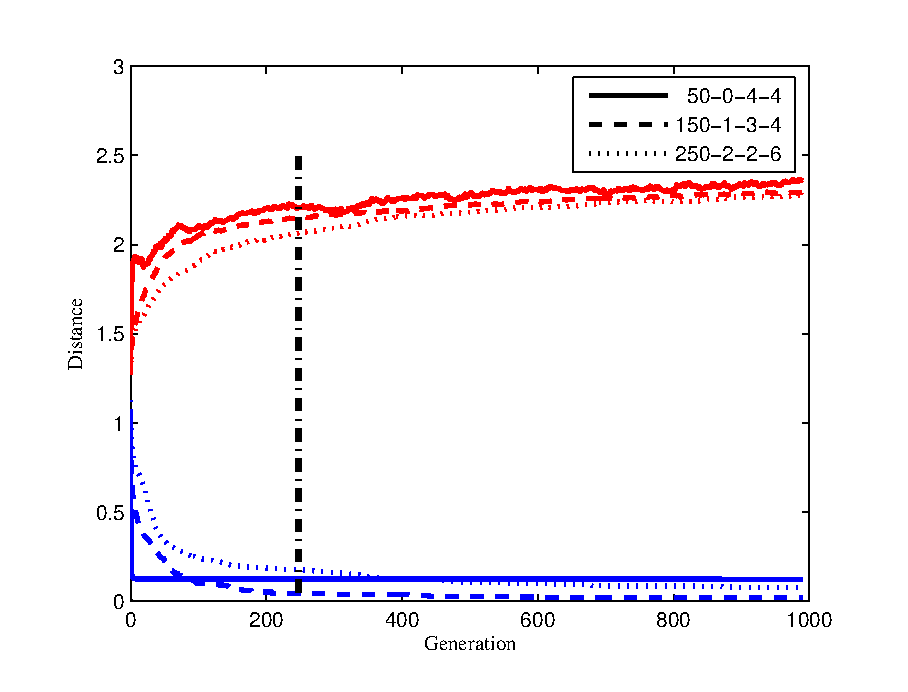
\includegraphics[height=4cm]{figures/parameter.eps}
\caption{标题}
\label{labeliiiiii}
\end{figure*}


\begin{table}
%\tiny 放不下把表格缩小
\centering
\caption{表名}
\label{tab:1}
% Table generated by Excel2LaTeX from sheet 'wilcoxon test4'
\begin{tabular}{l|c|c|c|c|c}
\hline
$11$    & $111$      & $11$+         & $11$-         & 11    & $\alpha$ = 0.05   \\
\hline
1 & 1/2& 458.0 & 70.0 & 1.2158E-4 & Y11ES \\ \hline
1& 301/1& 518.0 & 10.0 & 2.002E-8 & YE11S \\ \hline
1 & 11/8& 308.0 & 220.0 & $\geq$ 0.2 & 1NO \\ \hline
1 & 21/1& 518.0 & 10.0 & 2.002E-8 & YE111S \\ \hline
\hline

\end{tabular}%
\end{table}


\section{研究现状}

\section{本文工作}

\section{论文结构}

\clearpage{\pagestyle{empty}\cleardoublepage}       %本有
% !Mode:: "TeX:UTF-8"

\chapter{1}

\section{1}

\section{111}

\subsection{1111作}

\subsection{1111111作} %上交

\subsection{11}

\section{1111}

\section{111}


\section{本章小结}

\clearpage{\pagestyle{empty}\cleardoublepage}       %本有
% !Mode:: "TeX:UTF-8"

\chapter{C}

\section{算法架}

\subsection{研究动机}

\subsubsection{基本框架}


\section{本章小结}

\clearpage{\pagestyle{empty}\cleardoublepage}       %本有
\chapter{111}


\section{111}

\section{11}

\section{11}

\subsection{1}

\subsection{1}

\subsubsection{$I_{\epsilon+}$}


\section{xiaojie}





\clearpage{\pagestyle{empty}\cleardoublepage}       %本有
\chapter{总结与展望\label{conclusion}}


\section{11}

\clearpage{\pagestyle{empty}\cleardoublepage}       %本有

%%%%%%%%%%  参考文献  %%%%%%%%%%
\titleformat{\chapter}{\centering\sihao\hei}{\chaptername}{2em}{}
\defaultfont
%\bibliographystyle{TJUThesis}
\bibliographystyle{references/TJUThesis}        % bst文件名,注意不要后缀
\phantomsection
\markboth{参考文献}{参考文献}
\addcontentsline{toc}{chapter}{参考文献}        % 参考文献加入到中文目录
%\nocite{*}                                     % 若将此命令屏蔽掉,则未引用的文献不会出现在文后的参考文献中
\bibliography{references/reference}             % bib文件名
\include{references/reference}
\clearpage{\pagestyle{empty}\cleardoublepage}   %本有
% !Mode:: "TeX:UTF-8"



\markboth{附录A实验数据}{附录A~~实验数据}

\addcontentsline{toc}{chapter}{附录A~~验数据} % 添加到目录中
\chapter*{附录A~~实验数据}
\section*{附表标题}

\renewcommand{\tablename}{附表}                                     % 插表题头
%\renewcommand{\thetable}{\arabic{chapter}-\arabic{table}}         % 使表编号为 7-1 的格式
\renewcommand{\thetable}{A-\arabic{table}}         % 使表编号为 A-1 的格式
               %附录 实验结果表
\clearpage{\pagestyle{empty}\cleardoublepage}   %本有
\documentclass{llncs}

\usepackage{graphicx}
\usepackage{enumerate}
\usepackage{amsmath}
\usepackage{amssymb}
\usepackage{algorithm}
\usepackage{algorithmic}
\usepackage{multirow}
\usepackage{longtable}
\usepackage{indentfirst}
\allowdisplaybreaks[4]

\newcommand\etc{{\it et al.}}

\renewcommand{\algorithmicrequire}{\textbf{Input:}}
\renewcommand{\algorithmicensure}{\textbf{Output:}}
\renewcommand{\algorithmicreturn}{\textbf{Initialize:}}

\begin{document}

\title{Theorem Proving  of First-order Logic for Solving Pronoun Disambiguation Problems}
%\author{Yuhao Yang \and Yongmei Liu
%}
%\institute{
%Sun Yat-sen University \email{yangyh36@mail2.sysu.edu.cn}
%\and Sun Yat-sen University \email{ymliu@mail.sysu.edu.cn}
%}

\maketitle

\begin{abstract}
  In this paper, we propose theorem proving of first-order logic for solving pronoun disambiguation problems(PDP). The PDP task introduced in this paper contains the extended version of the publicly available questions in the Winograd Schema Challenge(WSC). To solve publicly available questions in the WSC, a question answering system must have the ability of finding the commonsense knowledde and reasoning out the answer based on the commonsense knowledge. To focus on the ability of reasoning out the answer, we build the extended version of publicly available questions in the WSC by manually adding related commonsense knowledge to each question. And then we build a question answering system using the algorithm of theorem proving of first-order logic. In result, our question answering system achieves 63.75\% accuracy, outperforming R-NET in the test set.


  \keywords{Winograd Schema Challenge(WSC), First-order Logic, Pronoun Disambiguation Problems, Logical Reasoning}

\end{abstract}

\section{Introduction}
\setlength{\parindent}{2em}In recent years, many systems which do not have the human-like intelligence have passed the Turing Test. Therefore, many possible Turing Test alternatives\cite{LevesqueDM12wsc}\cite{BringsjordBF01creativity}\cite{Riedl14lovelace} have been proposed. Among these possible alternatives, the Winograd Schema Challenge(WSC)\cite{Levesque11wsc}is proposed by Hector Levesque, a computer scientist at the university of Toronto. It is a multiple-choice test that employs questions of a very specific structure. Every Winograd Schema(WS) question is a pronoun disambiguation problem, which consists of three parts, description, question and answers pair. For example:\\
\par\indent	\textbf{Description:} The trophy doesn��t fit into the brown suitcase because it��s too small.\\
\indent	\textbf{Question:} What is too small?\\
\indent \textbf{Answers pair:} The trophy / the brown suitcase.\\
\par\indent To solve the example problem showed above is to find the word to replace ��what�� in the question sentence. As we know, if thing A is big and thing B is small, then thing A can��t fit into thing B. So, by substituting "thing A" with "the trophy" and substituting "thing B" with "the brown suitcase", we can reason that if the trophy is big and the brown suitcase is big, then the trophy dose not fit into the brown suitcase. And then we know that the correct answer to this question is ��the brown suitcase��. But for a machine, it might not have commonsense knowledge about the relationship between the word ��small�� and the phrase ��fit into��, and it dose not know how to use commonsense knowledge to reason out the correct answer. Therefore, the key to solve WS question is to find the commonsense knowledge related to the question and reason out the answer by using the commonsense knowledge. To solve WS question, Arpit Sharma et al. \cite{SharmaVAB15towards} used Google search to find the related commonsense knowledge and then used semantic parser to build the semantic representation graphs of the commonsense knowledge and the question. Finally, they reasoned on theses semantic representation graphs to find the answer. Among 282 WS questions, they select 71 pairs of the questions to solve and their system was able to answer 53 pairs. Quan Liu et al. \cite{LiuJLZWH16combing} proposed a commonsense knowledge enhanced embeddings model, which uses three knowledge base, WordNet\cite{Miller95wordnet}, ConceptNet\cite{Singh2004ConceptNetA}, CauseCom to search for commonsense knowledge related to the question and then uses the commonsense knowledge to learn knowledge enhanced embeddings. It achieves the best system with the highest accuracy 58.3\% in 2016 Winograd Schema Challenge. Both of these two methods use its own way to find commonsense knowledge and then use commonsense knowledge to reason out the answer, so theses two methods may get different number of correct commonsense knowledge related to the WS question and we can't explicitly tell which method has the better ability of reasoning. Therefore, we can manually add commonsense knowledge in the form of natural language for each WS question, which we call extended Winograd Schema(ExtWS) question.
\par\indent The ExtWS questions can be used to test a question answering system's ability of reading understanding and reasoning on natural language. To solve ExtWS questions, we proposed theorem proving of first-order logic algorithm and we got 63.75\% on 298 ExtWS questions and we used R-NET\cite{NETWORKS2017RnetMR} to solve ExtWS questions, and make a comparision between these two experiment results. R-NET ranked third on SQuAD and its source code is available on \url{https://github.com/YerevaNN/R-NET-in-Keras}.\\
\indent The remainder of the paper will start with introducing preparation of building our question answering system, which consists of three parts. First is to introduce the ExtWSC dataset and the next two part is to introduce two necessary tools which are used to build our question answering system. One of the tools is SEMPRE[9], which can be used as a semantic parser. The other is Z3-prover\cite{MouraB08z3},  a theorem prover, which we use to reason out the answer. Then we will introduce our approach, theorem proving of first-order logic. After that, we present the experiment result and analysis on solving ExtWSC. At last, we make conclusion and talk about our future work.

\section{Preparations}
In this section, we will introduce the ExtWSC dataset, semantic parser Sempre and theorem prover Z3.
\subsection{The ExtWSC Dataset}
The ExtWSC dataset includes 298 questions, each of which consist of description sentences, knowledge sentences, question sentences and answers pair. Compared with the WSC dataset, the ExtWSC dataset extends almost every question in the WSC dataset with one or more related commonsense knowledge sentences in the form of natural language. There are still some complicate questions which we don��t know how to add commonsense knowledge sentences for. Each commonsense knowledge sentence has the following form.\\
\indent	Commonsense knowledge sentence $->$ A $|$ If A, then B.\\
\indent	$S->$ one sentence with one verb and its related nouns\\
\indent $A->$ S $|$ S or A $|$ S and A\\
\indent $B->$ S $|$ S or B $|$ S and B\\

\noindent Each ExtWSC question has the following three forms.\\
\indent \textbf{One Sentence:} In the ExtWSC dataset, some questions are only related to one commonsense knowledge sentence and we human can reason out the answer by using this only one sentence.For example:\\
\indent	Description: The trophy doesn��t fit into the brown suitcase because it��s too small.\\
\indent	Knowledge: If thing A is big and thing B is small, then thing A can't fit into thing B.\\
\indent	Question: What is too small?\\
\indent	Answers pair: The trophy / the brown suitcase.\\

\indent \textbf{More Sentences:} There are also some questions related to more commonsense knowledge sentences and we can reason out the answer if and only if we use all these sentences.For example:\\
\indent	Description: The customer walked into the bank and stabbed one of the tellers. He was immediately taken to the emergency room.\\
\indent	Knowledge: If person B stabs person C, then person C might be hurt. If person B is hurt, then person B might be taken to emergency room.\\
\indent	Question: Who was taken to the emergency room?\\
\indent	Answers pair: The teller / the customer.\\

\indent \textbf{Complicate Questions:} There are still some questions which are too complicate to add commonsense knowledge sentences.For example:\\
\indent	Description: This book introduced Shakespeare to Goethe; it was a fine selection of his writing.\\
\indent	Question: Fine selection of whose writing?\\
\indent	Answers pair: Ovid /  Shakespeare\\
\indent To reason out the answer to this question, we must know who Shakespeare is and who Goethe is and there are no direct relations between the word ��introduced�� and the phrase ��selection of his writing��. Therefore, our system can not reason out the answer to such question.

\subsection{SEMPRE}
SEMPRE is a toolkit for training semantic parsers, which transform natural language texts to  intermediate logical forms. Its source code is available on \url{https://github.com/percyliang/sempre}, so we can download the source code on the github and then use script to run SEMPRE. In this paper, we use SEMPRE to parse sentences in ExtWSC questions. Its parsing result consists of three main parts. One is ��Lemmatized Tokens��, which shows all the lemmatized tokens in the sentence. Another one is ��POS tags��, identifying which word is a verb and which a word is noun and so on.  The last one is ��Dependency children��, identifying words�� relations in the sentence. For example, if we use SEMPRE to parse the sentence ��The trophy can��t fit into the brown suitcase��, we will know the subject of the phrase ��fit into�� is ��trophy�� and the object is ��suitcase��. Based on SEMPRE��s parsing result, our algorithm can automatically generate a Z3 script which can represent information about natural language sentence in first-order logic language. The Z3 script consists of several commands that can be executed by Z3-prover. We introduce this in next part.

\subsection{Z3-prover}
Z3-prover is a theorem prover from Microsoft Research. Its source code is available on \url{https://github.com/Z3Prover/z3}, so we can download the source code on the github and build it. In our algorithm, we use first-order logic language to represent sentences in the form of natural language. So we have to identify predicates and entities in the sentences. Then we transform proper names into individual constants and transform common nouns, verbs and adjectives into predicates. According to Z3 input format which is an extension of the one defined by the SMT-LIB 2.0 standard\cite{Barrett2010TheSS}, we can use the below commands in the Z3 script to represent natural language sentences. The ��declare-const�� command declares an individual constant, which represent a proper name in sentences . The ��declare-rel�� command declares a predicate, which represent a verb, a common noun or an adjective in sentences. Once we identify all the individual constants and predicates , we can use the ��assert�� command to represent a complete sentence in the form of first-order logic language. Then, we use Z3-prover to execute these command and get its resolving result. At last, we can reason out the answer to the ExtWSC question based on the result.

\section{Our Approach}
Our approach is based on two main tasks, namely, semantic parsing of natural language sentences, and introducing four auxiliary rules to reason out the answer. Next, we will explain how these two tasks help our question answering system to answer ExtWSC questions.
\subsection{Semantic Parsing of Natural Language Sentences}
In our algorithm, we use first-order logic language to represent natural language sentences, and use Z3 command to represent first-order logic language. Therefore, we firstly need to parse the natural language sentences. Here, we select SEMPRE as our semantic parser. Based on its parsing result, we use the following steps to automatically generate Z3 commands to represent first-order logic language information of natural language sentences.
\begin{enumerate}
\item \textbf{Identifying Individual Constants:} In first-order logic language, each individual constant refers to the entity in the sentences which bears that name. In natural language sentences, proper names can be translated into individual constants. For example, in sentence \emph{Joan made sure to thank Susan for all the help she had given}, the proper name \emph{Joan} is an individual constant. To automatically generate Z3 commands, once we identify a individual constant based on SEMPRE��s parsing result, we automatically add a Z3 command, \emph{(declare-const \%individualConstant \%sort)}, into the Z3 script. \%individualConstant is the string that represent the proper name in natural language sentences. \%sort is the sort that we use Z3 command \emph{declare-sort} to declare in Z3 script. Each individual constant must have a sort.

\item \textbf{Identifying Predicates:} In first-order logic language, each predicate refers to a verb, a common noun or an adjectives in the sentences. Predicates can have one or more arguments. Each argument is an individual constant or an individual variable. A predicate with n arguments is called n-place predicate. For example, in sentence \emph{Joan made sure to thank Susan for all the help she had given}, the verb phrase \emph{thank for} is a 3-place predicate with \emph{Joan, Susan, help} as arguments and \emph{(thankFor Joan Susan help)} is a proposition.

\item \textbf{Identifying Universal Quantifiers or Existential Quantifiers:} In ExtWSC questions, variables with universal quantifiers or existential quantifiers only exist in commonsense knowledge sentences. In our manually adding commonsense knowledge sentences, we add two constraints:\\
1.If a noun phrase consists of a word and an uppercase letter, it is a variable with universal quantifier which we use Z3 command \emph{forall} to declare.
2.If the word is \emph{something, somebody, he, him or it}, the word is a variable with existential quantifier which we use Z3 command \emph{exists} to declare.
Each variable with quantifiers also have a sort.

\item \textbf{Translating Description} After identifying all constants, predicates, variables in sentences, we add Z3 command, \emph{(assert (and (\%predicate1 \%constants1) (\%predicate2 \%constants2) ... ))}, into Z3 script, where \%predicate1 refer to the verb, common noun or adjective in the sentences and \%constants1 refer to all the proper names related to this predicate in the sentences. We use and to represent conjunction to make sure that each proposition is true.

\item \textbf{Translating Commonsense Knowledge} As we show above, there are two forms of commonsense knowledge sentences. For the sentence in the form of \emph{If A, then B.} ,we regard A as antecedent and B as consequent. And then add Z3 command to represent A entails B. For the sentence in the form of \emph{A} , we use the method similar to translating description sentences into Z3 commands.

\item \textbf{Translating Question} After translating description and commonsense knowledge sentences into Z3 commands, we need to translating question sentence to reason out the answer. Firstly identifying predicates and their arguments from question sentence. Secondly extracting question particle which has a tag \emph{WP} in SEMPRE��s parsing result. Finally replacing question particle with constants in answers pairs one by one and get its negative form. For example, in sentence \emph{Who had given help}, we add Z3 command \emph{(assert (not (give Joan help)))} and \emph{(assert (not (give Susan help)))} into different Z3 scripts.
\end{enumerate}
\subsection{Introducing Four Auxiliary Rules to Reason Out The Answer}
After automatically generating Z3 commands of sentences in description, commonsense knowledge and question, we still can��t reason out the correct answer to the ExtWSC question. Therefore, we introduce four auxiliary rules to reason out the correct answer.

\begin{itemize}
\item \textbf{Entity Inequality:} In 4.1, we use Z3 command declare-const to declare proper name in the sentences. From the view of script file, each proper name is represented by a string. But from the view of model, each proper name is just a value. Therefore, two different proper names represented by two different string may have the same value, which may make our system to reason out a wrong answer. So we add the rule of entity inequality for the individual constants that have the same sort. For example, in the sentence Joan made sure to thank Susan for all the help she had given, we firstly get two individual constants Joan and Susan, and then we add Z3 command (assert (not (= Joan Susan))).
\item \textbf{Closed-world Assumption:} According to closed-world assumption, everything we don��t know is false. Therefore, for variables with existential quantifier or universal quantifier, we must limit the range of them so that these variables can only take the value of the individual constants which have been identified in the ExtWSC question. For example, in the sentence Joan made sure to thank Susan for all the help she had given, we firstly declare two individual constants with Z3 commands (declare-const Joan person) and (declare-const Susan person), and then we add Z3 command (assert (forall ((x person)) (or (= x Joan) (= x Susan)))), to limit the range of x when x has the sort person.

\item \textbf{Closed-reason Assumption:} In our approach, we reason out the correct answer when the propositions in description sentences entail the proposition in question sentence.According to our manually adding commonsense knowledge sentences, sometimes the propositions in description sentences are antecedent in an entailment and sometimes the propositions in question sentence are antecedent. Therefore, we introduce closed-reason assumption.\\
    Assuming the question sentence has the predicates (Q1) or (Q1 and Q2) and the description sentences have the predicates (D1) or (D1 and D2). In an entailment of commonsense knowledge sentences, Q1 and Q2 have the following relations with D1 and D2.
    \begin{enumerate}
    \item Q1 and Q2 in the antecedent: 
    \\if Q1 entails (D1 and D2), we add sentences, D1 entails Q1, D2 entails Q1; 
    \\if Q1 entails (D1 or D2), we add sentences, D1 entails Q1, D2 entails Q2; 
    \\if (Q1 or Q2) entails D1, we add sentences, D1 entails Q1, D1 entails Q2; 
    \\if (Q1 and Q2) entails D1, we add a sentence, D1 entails (Q1 and Q2); 
    \\if Q1 entails D1, we add a sentence, D1 entails Q1.
    \item Q1 and Q2 in the consequent: 
    \\if D1 entails (Q1 or Q2), we add two sentences, D1 entails Q1, D1 entails Q2; 
    \\for other relations, we add one sentence, consequent entails antecedent.
    \end{enumerate}
\item \textbf{Unique Answer:}Each ExtWSC question has only one correct answer, so we add Z3 command to assure that once candidate answer A is the correct answer, candidate answer B can not be the correct answer.
\end{itemize}
\section{Experiments}
\subsection{Accuracy}
In this paper, we aim to test if our question answering system has the better ability of reasoning in ExtWSC questions than R-NET. Among 298 ExtWSC questions, our system can correctly answer 105 questions, while R-NET can only answer 60 questions. Because every ExtWSC question has two candidate answers, both of these two systems can randomly select one of the candidate answers as their output. We add the ability of randomly selecting candidate answer into these two systems when the systems can not reason out the answer. In result, our system achieves 63.75\% accuracy while R-NET achieves 55.03\% accuracy.\\
\begin{table}
\centering
\caption{Experiment results of two approaches. The random-guess accuracy for this dataset is 44\%}
\begin{tabular}{|l|c|r|}
\hline
Approach&Num of Solved Problem&Accuracy with Guessing\\
\hline
ours&105&63.75\%\\
\hline
R-NET&60&55.03\%\\
\hline
\end{tabular}
\end{table}

\subsection{Error Analysis}
Although we manually add commonsense knowledge sentence for each WS question to get ExtWSC questions, we still can��t achieve 90\% accuracy on ExtWSC questions. We conclude three reasons why our system can��t reason out the correct answer. Firstly, our semantic parsing tool SEMPRE can not correctly find the predicate and its related entities in those sentences which have attributive clause or appositive clause, so we can not generate a correct Z3 script for such sentences. Secondly, some words, which should be parsed as verb, are parsed as noun or adjective. Therefore, our system gets wrong words�� dependency and then gets wrong predicates or wrong entities. Thirdly, some WS questions are so complicate that we can��t add related commonsense knowledge sentences for them and our system can��t reason out the answer without commonsense knowledge.
\section{Conclusion and Future Works}
In this paper, by adding commonsense knowledge sentences for every WS question, we build a new dataset, which is called ExtWSC questions. ExtWSC questions can be used to test a question answering system��s ability of reading comprehension and reasoning out the answer. Then, we propose theorem proving of first-order logic to build a question answering system. In this algorithm, we firstly propose how to translate natural language sentence into a Z3 script, which can represent first-order logic formula. Secondly, we introduce four auxiliary rules to complete a Z3 script to make it possible to reason out the answer. Finally, we compare our system with R-NET. In result, our question answering system outperforms R-NET in accuracy.\\
\indent Although our question answering system outperforms R-NET, it still can not achieve 90\% accuracy. As error analysis shows, there exist some sentences that can��t be correctly parsed by SEMPRE. Therefore, in our future work, we will use coreference resolution tool in NLTK, dependency parser and SEMPRE altogether to parse a sentence and get the predicates and entities more accurately. Besides, our system relies on manually added commonsense knowledge to reason out the answer. So we will aim to solve WS question which doesn��t contain the commonsense knowledge sentences by automatically extracting the related commonsense knowledge in ConceptNet, WordNet, CauseCom or ResearchCyc\cite{Matuszek2006cyc}.

\bibliographystyle{splncs}
\bibliography{paper}
\end{document}
                       % 攻读硕士学位期间发表学术论文情况
\clearpage{\pagestyle{empty}\cleardoublepage}   %本有
% !Mode:: "TeX:UTF-8"

%\titlecontents{chapter}[2em]{\vspace{.5\baselineskip}\xiaosan\song}
%             {\prechaptername\CJKnumber{\thecontentslabel}\postchaptername\qquad}{}
%             {}                            % 设置该选项为空是为了不让目录中显示页码
%\fancypagestyle{plain}   % 设置页眉页脚风格,按照教务处规定,此处出现页眉,但是没有页脚(页码)。
%\lhead{}

%\lhead{\song\wuhao 中山大学硕士学位论文}  % 左页眉
%\rhead{\song\wuhao \leftmark}
%\chead{\song\wuhao 中山大学硕士学位论文} % 设置页眉内容
%\lfoot{}
%\cfoot{\song\xiaowu~\thepage~}
%\rfoot{}
\markboth{致\quad 谢}{致\quad 谢}
\addcontentsline{toc}{chapter}{致\quad 谢} % 添加到目录中
\chapter*{致\quad 谢}
             % 致谢
\clearpage{\pagestyle{empty}\cleardoublepage}
\clearpage
\end{CJK*}                                      % 结束中文字体使用
\end{document}                                  % 结束全文
